%%%%%%%%%%%%%%%%%%%%%%%%%%%%%%%%%%%%%%%%%
% Journal Article
% LaTeX Template
% Version 1.4 (15/5/16)
%
% This template has been downloaded from:
% http://www.LaTeXTemplates.com
%
% Original author:
% Frits Wenneker (http://www.howtotex.com) with extensive modifications by
% Vel (vel@LaTeXTemplates.com)
%
% License:
% CC BY-NC-SA 3.0 (http://creativecommons.org/licenses/by-nc-sa/3.0/)
%%%%%%%%%%%%%%%%%%%%%%%%%%%%%%%%%%%%%%%%%

%----------------------------------------------------------------------------------------
%	PACKAGES AND OTHER DOCUMENT CONFIGURATIONS
%----------------------------------------------------------------------------------------

\documentclass[twoside,twocolumn]{article}

\usepackage{blindtext} % Package to generate dummy text throughout this template

\usepackage[sc]{mathpazo} % Use the Palatino font
\usepackage[T1]{fontenc} % Use 8-bit encoding that has 256 glyphs
\linespread{1.05} % Line spacing - Palatino needs more space between lines
\usepackage{microtype} % Slightly tweak font spacing for aesthetics

\usepackage[german]{babel} % Language hyphenation and typographical rules

\usepackage[hmarginratio=1:1,top=32mm,columnsep=20pt]{geometry} % Document margins
\usepackage[hang, small,labelfont=bf,up,textfont=it,up]{caption} % Custom captions under/above floats in tables or figures
\usepackage{booktabs} % Horizontal rules in tables

\usepackage{lettrine} % The lettrine is the first enlarged letter at the beginning of the text

\usepackage{enumitem} % Customized lists
\setlist[itemize]{noitemsep} % Make itemize lists more compact

\usepackage{abstract} % Allows abstract customization
\renewcommand{\abstractnamefont}{\normalfont\bfseries} % Set the "Abstract" text to bold
\renewcommand{\abstracttextfont}{\normalfont\small\itshape} % Set the abstract itself to small italic text

\usepackage{titlesec} % Allows customization of titles
\renewcommand\thesection{\Roman{section}} % Roman numerals for the sections
\renewcommand\thesubsection{\roman{subsection}} % roman numerals for subsections
\titleformat{\section}[block]{\large\scshape\centering}{\thesection.}{1em}{} % Change the look of the section titles
\titleformat{\subsection}[block]{\large}{\thesubsection.}{1em}{} % Change the look of the section titles

\usepackage{fancyhdr} % Headers and footers
\pagestyle{fancy} % All pages have headers and footers
\fancyhead{} % Blank out the default header
\fancyfoot{} % Blank out the default footer
\fancyhead[C]{Evolutionäre Optimierungsalgorithmen $\bullet$ MK - Einführung in das wissenschaftliche Arbeiten} % Custom header text
\fancyfoot[RO,LE]{\thepage} % Custom footer text

\usepackage{titling} % Customizing the title section

\usepackage{hyperref} % For hyperlinks in the PDF

\newcommand{\e}[1]{\times 10^{#1}}

\usepackage{graphicx}

\usepackage{amsmath}

\usepackage{csquotes}

%----------------------------------------------------------------------------------------
%	TITLE SECTION
%----------------------------------------------------------------------------------------

\setlength{\droptitle}{-4\baselineskip} % Move the title up

\pretitle{\begin{center}\Huge\bfseries} % Article title formatting
\posttitle{\end{center}} % Article title closing formatting
\title{Evolutionäre Optimierungsalgorithmen} % Article title
\author {
	\textsc{Federico Ramírez Villagrana} \\[1ex]
	\normalsize Universität Hamburg \\
	\normalsize Methodenkompetenz - Einführung in das wissenschaftliche Arbeiten \\
	\normalsize Dozent: Dr. Andreas Günther
}
\date{} % Leave empty to omit a date
\renewcommand{\maketitlehookd}{%
\begin{abstract}
\noindent In diesem Paper wird darüber diskutiert, sowohl was Optimierung ist und warum ist es schwer, als auch was evolutionäre Algorithmen (EA) sind und wie, warum,  und wann sind sie hilfreich im Optimierung-Bereich. Es wird auch im Detail erklärt, wie EA funktionieren und warum sind sie als teil der künstlichen Intelligenz betrachtet. Es werden auch einige bekannte EA erwähnt und oberflächlich erklärt. Am ende wird darüber diskutiert, welche     Vor- und Nachteile die EA haben.
\end{abstract}
}

%----------------------------------------------------------------------------------------

\begin{document}

% Print the title
\maketitle

%----------------------------------------------------------------------------------------
%	ARTICLE CONTENTS
%----------------------------------------------------------------------------------------

\section{Einleitung}
\lettrine[nindent=0em,lines=3]{D} as Problem des Handlungsreisenden (engl. traveling salesman problem oder TSP) ist ein sehr bekanntes und studiertes Problem im Informatik-Bereich. Es geht wie folgendes:\par
Eine Reihenfolge für den Besuch mehrerer Orte muss so gewählt sein, dass keine Station außer der ersten mehr als einmal besucht wird, die gesamte Reisestrecke des Handlungsreisenden möglichst kurz, und die erste Station gleich der letzten Station ist. \cite{wiki_tsp}\par
Sei $n$ die Anzahl der Stationen, dann es $(n-1)!$ mögliche Lösungen für das TSP gibt. Daher wenn $n=4$, dann es $6$ mögliche Lösungen gibt. Es ist nicht schwer, einen brute-force \footnote{Auch Exhaustionsmethode, ist eine Lösungsmethode für Probleme, die auf dem Ausprobieren aller möglichen (oder zumindest vieler möglicher) Fälle beruht. \cite{wiki_brute_force}} Ansatz zu verfolgen, für ein Problem, das nur 6 Lösungen hat. Aber wenn $n=50$, dann es circa $6,1\e{62}$ Lösungen gibt.\par
Folgendes ist hilfreich, um diese Anzahl in einer Perspektive zu setzen: Das Universum ist circa 15 Milliarde Jahre alt, das ist $4,7\e{17}$ Sekunden. Wenn es eine Billion Rechner gäbe, die jede einzeln seit dem Anfang des Universums eine Billion Lösungen pro Sekunde berechnete, bisher wären nur $4,7\e{41}$ Lösungen berechnet worden.\par
Das TSP ist nur ein Beispiel von vielfältigen Problemen, die zu den kombinatorischen Problemen gehören, das heißt, Probleme, für die kein brute-force Ansatz möglich ist. In diesem Fall sind evolutionärer Algorithmen (EA) ein gutes Werkzeug, um gute Lösungen zu finden.\par
Natürlich können wir nicht sicher sein, dass wir die beste Lösung gefunden haben, außer wenn wir jede mögliche Lösung berechnet haben. Aber wie mit dem TSP-Beispiel gezeigt worden, ist es jedoch nicht immer möglich, alle mögliche Lösungen (in angemessener Zeit) zu berechnen.

%------------------------------------------------

\section{Stand der Forschung}
\lettrine[nindent=0em,lines=3]{I} n den 70ern Jahren wurde erstmals über EA diskutiert. Die erste Form von EA waren die genetische Algorithmen, die in \cite{holland_ga} eingeführt würden. Seit damals wurden jedes Jahr mehrere EA präsentiert. Es ist auch üblich, dass nicht nur Varianten von schon bekannten EA eingeführt werden, sondern auch neue Anwendungen. In \cite{algorithmen_list} allein werden circa 48 EA gelistet.\par
Heutzutage finden sich immer mehr Anwendungen der EA in nahezu allen Bereichen. Von der Medizin \cite{ea_und_medizin} und Biologie \cite{ea_und_biologie} über das Motor- \cite{ea_und_motoren} und Flugzeugdesign \cite{ea_und_flugzeuge_a} \cite{ea_und_flugzeuge_b} bis hin zur Kunst \cite{ea_und_kunst_a} \cite{ea_und_kunst_b} und Wirtschaft \cite{ea_und_wirtschaft}.

%------------------------------------------------

\section{Optimierung}
\lettrine[nindent=0em,lines=3]{I} m Mathematik-Bereich bedeutet Optimierung, die Findung von Parametern eines Systems, die ein bestmögliches Ergebnis erzielen. \cite{wiki_optimierung} Wir können diese Findung von Parametern auch wie folgendes definieren: Die Auswahl der bestmöglichen Lösung eines Problems von einer Menge möglicher Lösungen.\par
In Optimierungsprobleme wird eine Zielfunktion (engl. objective function) definiert, die entweder maximiert oder minimiert werden soll. Die Zielfunktion wird \enquote{Kosten-Funktion} oder \enquote{Fitness-Funktion} in Minimierung- und Maximierungsprobleme beziehungsweise genannt.\par
Sei $f(x)$ eine Zielfunktion, dann $x$ ein Vektor ist, der \enquote{Entscheidungsvariable} genannt wird. Die Anzahl von Elementen in $x$ wird die \enquote{Dimension} des Problems genannt.
Die Domäne der Zielfunktion repräsentiert die mögliche Lösungen des Problems. \par
Das Ziel der Optimierung ist es denn, die bestmögliche Lösung des Problems zu finden, das heißt, einen Wert für die Entscheidungsvariable zu finden, sodass die Zielfunktion einen Maximal- beziehungsweise Minimalwert ergibt.\par
Es gibt verschiedene Klassifizierungen oder Arten von Optimierung:

\begin{itemize}
\item{Eingeschränkte Optimierung - Die Entscheidungsvariable kann nicht irgendwelchen Wert aus der Domäne der Zielfunktion nehmen. Es gibt Einschränkungen dafür.}
\item{Multi-objective Optimierung - Das Problem besteht aus vielfältigen Zielfunktionen.}
\item{Multi-modale Optimierung - Die Zielfunktion hat mehrere Minima bzw. Maxima. Abbildung \ref{fig:rastrigin} zeigt eine multi-modale Funktion.}
\end{itemize}

\begin{figure}
\caption{Rastrigin function. Quelle: \url{https://commons.wikimedia.org/wiki/File:Rastrigin_function.png}}
\label{fig:rastrigin}
\centering
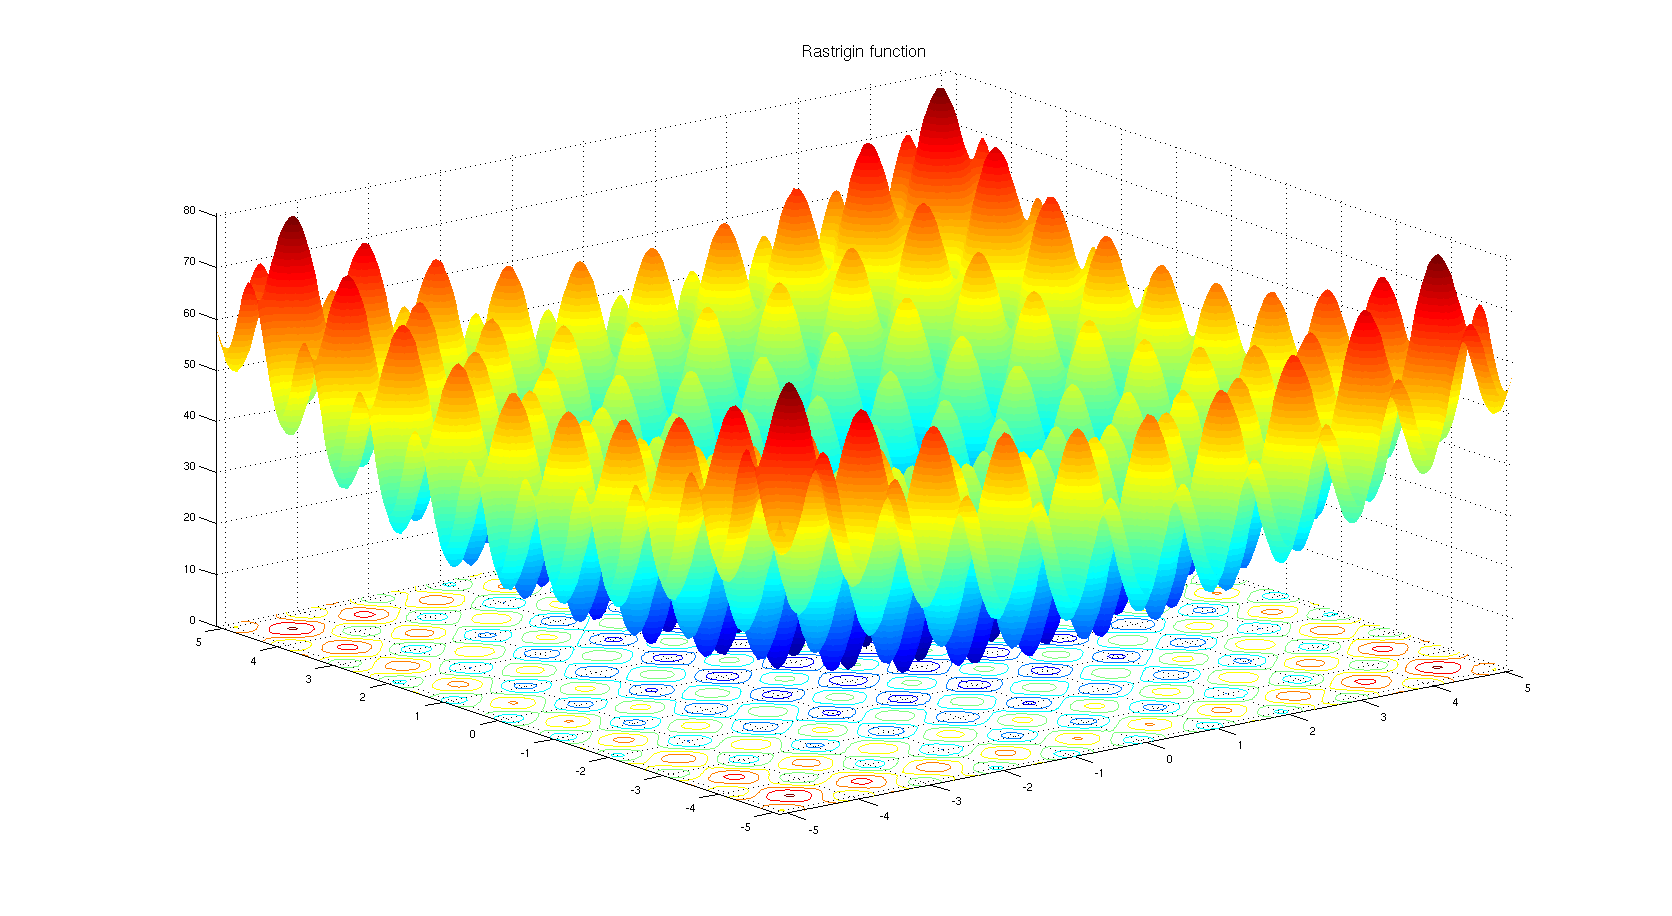
\includegraphics[width=0.5\textwidth]{images/rastrigin_function.png}
\end{figure}

Eine der wichtigsten und schwierigsten Teile der Optimierung ist es, eine geeignete Zielfunktion zu definieren, die die wichtige zu optimierenden Faktoren berücksichtigt.
Probleme im wirklichen Leben sind normalerweise eingeschränkt, multi-Objectiv und multi-modal, oder mit einer großen Anzahl von Dimensionen. Wegen dieser Eigenschaften der Zielfunktionen und der Optimierungsprobleme ist es schwierig, eine gute Lösung mittels traditioneller Vorgänge zu finden. Im Laufe der Zeit haben EA sich als gutes Werkzeug zur Lösung dieser Art von Probleme in angemessener Zeit erwiesen.

%------------------------------------------------

\section{Was ist ein evolutionärer Algorithmus?}
\lettrine[nindent=0em,lines=3]{D} er EA-Bereich ist ziemlich neu, deswegen gibt es bisher keine allgemein akzeptierte Definition von evolutionären Algorithmus.\par
EA sind zwar als Teil der künstliche Intelligenzes (KI) betrachtet, aber genau wo sie in Verbindung mit anderen KI-Methoden stehen, und was der EA-Bereich beinhaltet, ist von dem Autor abhängig. Abbildung \ref{fig:metaheuristics} zeigt eine von mehreren möglichen Klassifikationen von KI-Methoden in Bezug auf Metaheuristics (welche über den Rahmen dieses Papiers hinausgehen).

\begin{figure}
\caption{Klassifikation von Metaheuristics. Quelle: \url{https://en.wikipedia.org/wiki/File:Metaheuristics_classification.svg}}
\label{fig:metaheuristics}
\centering
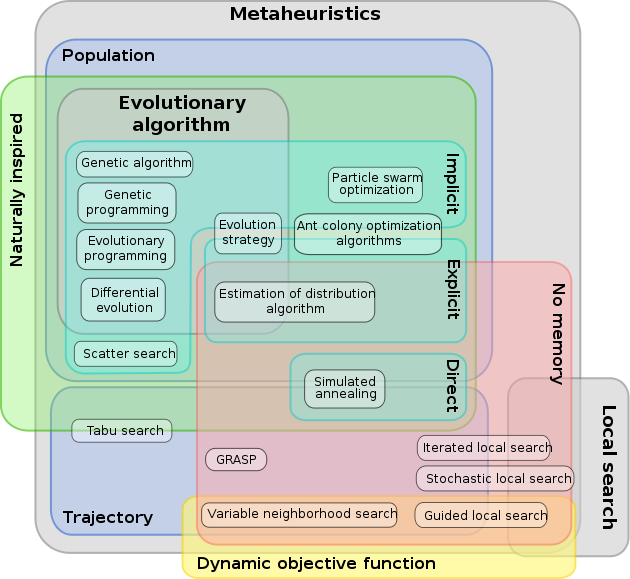
\includegraphics[width=0.5\textwidth]{images/metaheuristics_classification.png}
\end{figure}

In Abbildung \ref{fig:metaheuristics} kann auch erkannt werden, dass der Autor Particle Swarm Optimization (PSO) und Ant Colony Optimization (ACO) nicht als EA betrachtet. Trotzdem gibt es andere Autoren (wie z. B. \cite{wiley_evolutionary}), die diese Algorithmen genau für EA halten.\par

In diesem Paper wird folgende Definition für evolutionäre Algorithmus genommen: Ein Algorithmus, der die Lösung eines Problems durch viele Iterationen entwickelt    .

\subsection{Eigenschaften der evolutionären Algorithmen}
Folgende sind die Hauptelemente, die ein Algorithmus haben soll, um er als \enquote{evolutionär} zu betrachten:

\begin{itemize}
\item{Eine Zielfunktion.}
\item{Eine sogenannte Bevölkerung von mögliche Lösungen - Eine Menge von Darstellungen der Lösungen (Elemente der Domäne der Zielfunktion) des Problems, die mittels des Algorithmus und mehreren Iterationen (auch \enquote{Generationen} genannt) verarbeitet und hoffentlich verbessert werden.}
\item{Vorgänge, die die Elementen der Bevölkerung betreffen und verändern.}
\end{itemize}

Die meisten EA sind aus der Natur inspiriert, das heißt, dass Wissenschaftler Ereignisse, Systeme, und Mechanismen der Natur beobachten und danach versuchen einigermaßen, sie mit Algorithmen zu reproduzieren. EA werden \enquote{evolutionär} genannt, denn sie sind ursprünglich auf die Evolution basiert. \cite{holland_ga}

\subsection{Eigenschaften der Intelligenz}
Wie vorher gesagt, EA sind als Teil der KI betrachtet, weil sie Eigenschaften intelligenter natürlicher Systeme emulieren.\par
Laut \cite{wiley_evolutionary} sind die folgenden Eigenschaften notwendig, um ein System als intelligent zu betrachten:

\begin{itemize}
\item{Adaptation - Ein intelligentes System muss in hohem Maße an unvorhersehbare Änderungen anpassbar sein. Lernen ist daher unerlässlich.}
\item{Zufälligkeit - Obwohl Zufälligkeit meistens als eine schlechte Eigenschaft betrachtet wird, ist es in gewissem Maße notwendig, damit neue Lösungen eines Problems gefunden werden können.}
\item{Kommunikation -  Zwar wird eine einzige Ameise nicht wirklich als intelligent beurteilt, aber eine Ameisenkolonie wird (dank Kommunikation durch Pheromone) als eine super-intelligente Einheit überlegt.}
\item{Rückmeldung - Ein System kann sich nicht anpassen und verbessern, wenn es seine Umgebung nicht erkennen und darauf reagieren kann. Auch um zu lernen, muss ein System seine Fehler (mittels Rückmeldung) erkennen.}
\item{Erkundung - Das heißt, neue Lösungen finden, neue Wege erkunden, neue Ideen erzeugen. Normalerweise ist Erkundung eng mit Zufälligkeit verbindet.}
\item{Ausbeutung - Der Gegenteil von Erkundung. Das heißt, schon bekannte Lösungen und Wege (oder Kenntnisse) ausnutzen.}
\end{itemize}

In nächster Sektion werden verschiedene Beispiele von EA gezeigt und in jedem Beispiel wird erwähnt, welches Teil des Algorithmus welche Eigenschaft der Intelligenz versucht zu emulieren. Es ist auch wichtig zu nennen, dass nicht jede Eigenschaft des Intelligenzes von jeden EA repliziert ist.

%------------------------------------------------

\section{EA Beispiele}
\lettrine[nindent=0em,lines=3]{H} eutzutage gibt es viele EA und jedes Jahr werden neue entwickelt. In dieser Sektion werden nur ein paar der bekanntesten und wichtigsten erwähnt und oberflächlich erklärt.

\subsection{Genetische Algorithmen}
Genetische Algorithmen (engl. genetic algorithms oder GA) sind ursprünglich in \cite{holland_ga} präsentiert und danach in \cite{goldberg_ga} weiterentwickelt. Der Name \enquote{Genetic Algorithms} bezieht sich mehr auf eine Familie von Algorithmen als auf einen einzigen Algorithmus.\par
GA sind die erste vorgestellten, bekanntesten, und am meisten verwendeten EA. Ursprünglich waren sie dafür entwickelt, um adaptierbare Systeme zu studieren. Sie sind Simulationen der natürlichen Selektion. Daher sind sie genau auf die Evolution basiert.\par
Es gibt sechs Hauptteile der GA:

\begin{enumerate}
\item{Codierung der Lösungen - Als erstes muss man eine geeignete Codierung für die möglichen Lösungen finden. Das heißt, eine Darstellung für die Lösungen finden, die einfach zu verarbeiten ist. Eine die am meisten verwendeten Codierungen ist eine Bit-Folge. In dieser Codierung jedes Bit wird \enquote{Gen} genannt.}
\item{Ursprüngliche Bevölkerung - Eine ursprüngliche Bevölkerung muss initialisiert werden. Diese Initialisierung kann entweder zufällig oder auf Vorkenntnis basiert sein. Wie viele Elemente die Bevölkerung hat, ist ein wichtiger Parameter. Je mehr Elemente es gibt desto höher die Wahrscheinlichkeit, um gute Lösungen zu finden.}
\item{Fitnessfunktion - Die Zielfunktion des Problems. Der Wert, den ein Element der Bevölkerung darstellt, wird die Eingabe für die Zielfunktion. Der Wert, den die Zielfunktion ergibt, wird die \enquote{Fitness} des Elements genannt.}
\item{Auswahl von Einzelnen - Zwei Elemente der Bevölkerung werden ausgewählt, um ein neues Element herzustellen. Das verfolgte Verfahren, um die Elemente auszuwählen, kann entweder zufällig sein, oder auf die Fitness der Elemente basiert. Die ausgewählten Elemente werden \enquote{Eltern} genannt.}
\item{Crossover - Dies ist der wichtigste Teil der GA. Es definiert wie das neue Element aus die Eltern erstellt wird. Das heißt, welche Gene wird das neue Element von jeden Elternteil erben.}
\item{Mutation - Einige zufälligerweise-ausgewählte neu-erstellte Elemente werden mutiert. Das heißt, dass einige Bits gekippt werden. Welche Elemente mutiert werden und wie viele und welche Bits gekippt werden, kann mittels verschiedener Verfahren beziehungsweise entscheidet werden.}
\end{enumerate}

\begin{figure}
\caption{Wesentlich genetic Algorithmen pseudo-Code. Quelle: \cite{wiley_evolutionary}}
\label{fig:ga_pseudo}
\centering
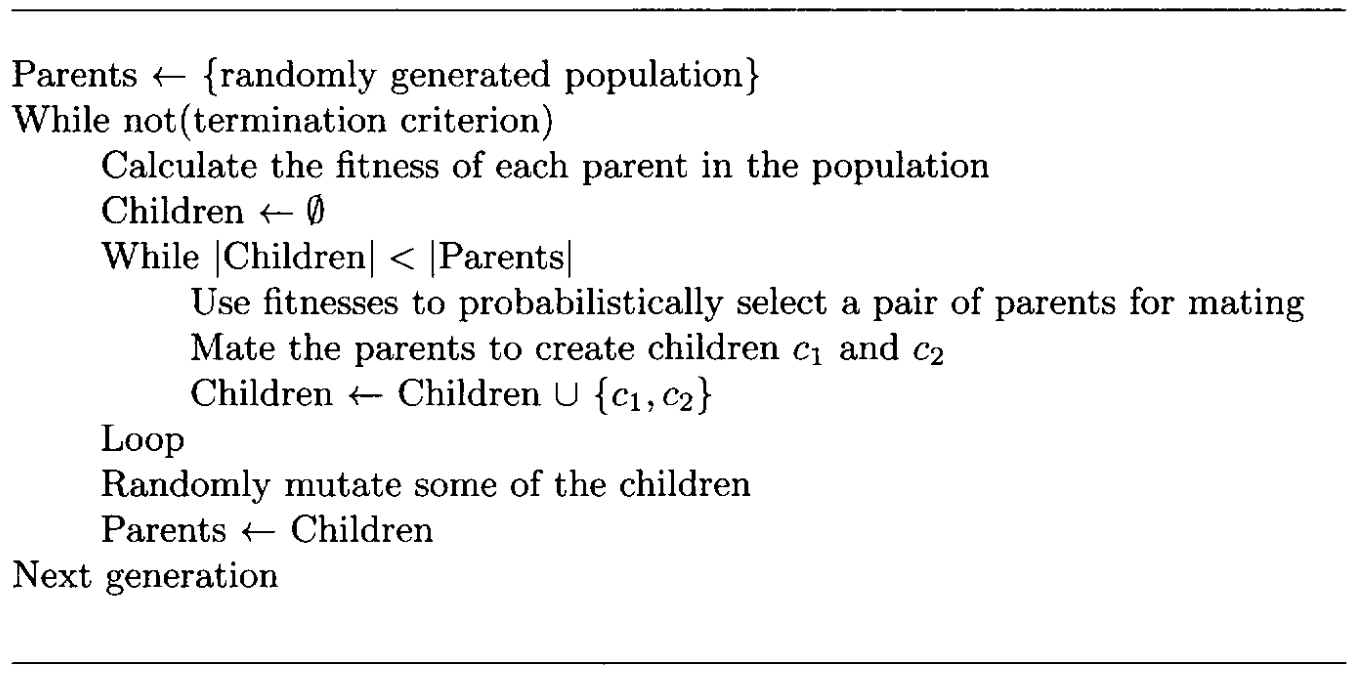
\includegraphics[width=0.5\textwidth]{images/ga_pseudo.png}
\end{figure}

EA insgesamt sind Problem-unabhängig, das heißt, dass wenn es eine geeignete Darstellung der Lösungen und eine geeignete Zielfunktion gibt, kann theoretisch jedes Problem mittels EA optimiert werden. Aus diesem Grund gibt es bei jeden EA ein Element der \textbf{Adaptation}.\par
In 2. Teil sowie in 4. bis 6. Teilen kann \textbf{Zufälligkeit} verwendet werden, je nachdem welche Verfahren jeweils ausgewählt werden.\par
In dem Mutation-Teil, eine hoch Wahrscheinlichkeit, um Elemente zu mutieren, heißt viel \textbf{Erkundung} und weniger \textbf{Ausbeutung}, und umgekehrt.

\subsection{Partikelschwarmoptimierung}
Partikelschwarmoptimierung (engl particle swarm optimization oder PSO) wird ursprünglich in \cite{kennedy_pso} und in \cite{shi_pso} präsentiert.\par
PSO ist auf menschlichen sozialen Verhalten basiert. \cite{eberhart_pso} Genauer,  PSO basiert auf der Beobachtung von Gruppen von Individuen, die zusammenarbeiten, um nicht nur ihr kollektives Verhalten in einer bestimmten Aufgabe zu verbessern, sondern auch ihr individuelles Verhalten zu verbessern.\par
Die Grundideen hinter PSO sind die folgende:

\begin{itemize}
\item{Es gibt eine Menge Partikeln, die sich mit einer beliebigen Geschwindigkeit durch den Suchraum bewegen.}
\item{Der Suchraum wird in \enquote{Nachbarschaften} mit einer beliebigen gleichen Größe unterteilt.}
\item{Jeder Partikel speichert sowohl die beste Position, die sie im Suchraum besucht hat, als auch die beste Position, die ihre Nachbarn erreicht haben.}
\item{Beide die Partikels beste Position und ihre Nachbarns beste Position beeinflussen die Partikels Geschwindigkeit.}
\end{itemize}

\begin{figure}
\caption{Wesentlich PSO Algorithmus pseudo-Code. Quelle: \cite{wiley_evolutionary}}
\label{fig:pso_pseudo}
\centering
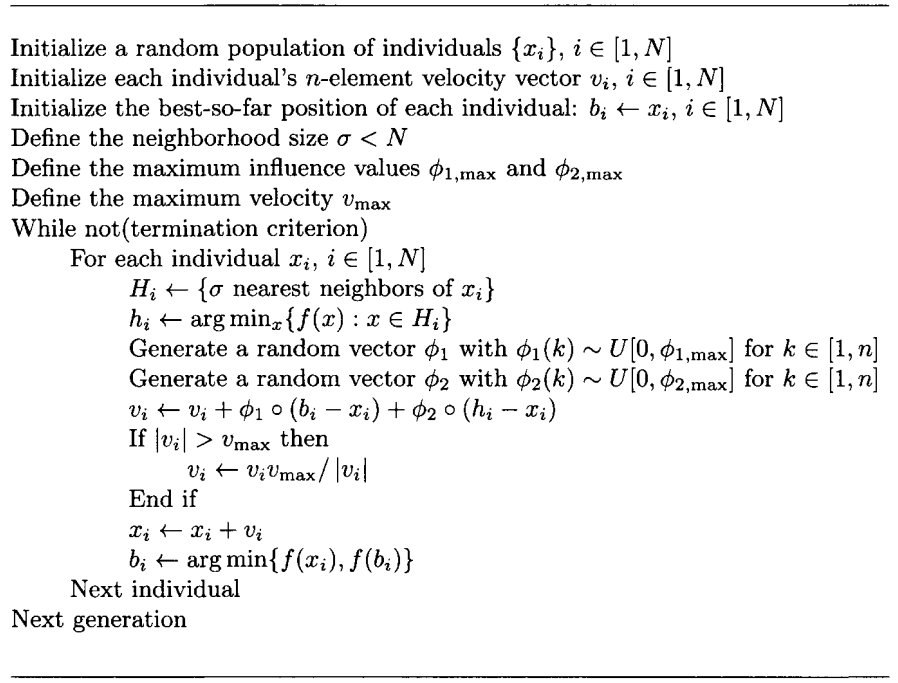
\includegraphics[width=0.5\textwidth]{images/pso_pseudo.png}
\end{figure}

In PSO können die Geschwindigkeiten der ersten Bevölkerung zufällig initialisiert werden. Daher gibt es ein Element der \textbf{Zufälligkeit}.\par
Da die Partikeln die besten bisher erreichten Positionen ihrer Nachbarn kennen muss, gibt es auch \textbf{Kommunikation}.\par
\textbf{Rückmeldung} wird verwendet, indem die besten bisher erreichten Positionen die Geschwindigkeit der Partikel beeinflussen. In welchen Ausmaß wird die Partikel beeinflusst, kann entweder \textbf{Erkundung} oder \textbf{Ausbeutung} fördern.

\subsection{Differenziale Evolution}
Differenziale Evolution (engl. differential evolution oder DE) wurde erstmals in \cite{storn_de_a} und \cite{storn_de_b} erwähnt. Aber die erste vielfach gelesene DE-Veröffentlichung war \cite{price_storn_de}.\par
Im Gegensatz zu fast alle anderen EA, DE ist nicht auf der Natur inspiriert. Eine der wichtigsten Merkmale der DE ist, dass es einfach ist. Dies Merkmal ist wichtig, da es Benutzer aus anderen Bereiche (d. h. nicht Informatikern/inen oder Mathematiker/inen) erlaubt, es umzusetzen.\par
Die wesentliche Schritte eines DE Algorithmus sind die folgende:

\begin{enumerate}
\item Die Bevölkerung eines DE Algorithmus besteht auf Vektoren mit $n$ Elemente. Wo $n$ die Dimension des Problems ist. Weiterhin, jeder Vektor selbst stellt eine mögliche Lösung des Problems dar.
\item Zwei Vektoren $x_{r2}, x_{r3} \mid r2 \neq r3$ werden ausgewählt.
\item Die Differenz zwischen $x_{r2}$ und $x_{r3}$ wird berechnet.
\item Die skalierte Differenz wird zu einem dritten Vektor $x_{r1} \mid r1 \notin \{ r2, r3 \}$ addiert. Dies wird eine neue mögliche Lösung $v_i$ ergeben.
\item $v_i$ wird mit einem Vektor $x_i \mid i \notin \{ r1, r2, r3 \}$ kombiniert.
\item $x_i$ wird gegen $u_i$ vergleicht und nur der beste wird behaltet.
\end{enumerate}

Abbildung \ref{fig:de_beispiel} zeigt 2. bis 4. Schritte für ein Problem mit 2 Dimensionen. Abbildung \ref{fig:de_pseudo} zeigt einen kompletten DE Algorithmus pseudo-Code für $n$ Dimensionen.\par

\begin{figure}
\caption{Grundlegende Idee von DE. Quelle: \cite{wiley_evolutionary}}
\label{fig:de_beispiel}
\centering
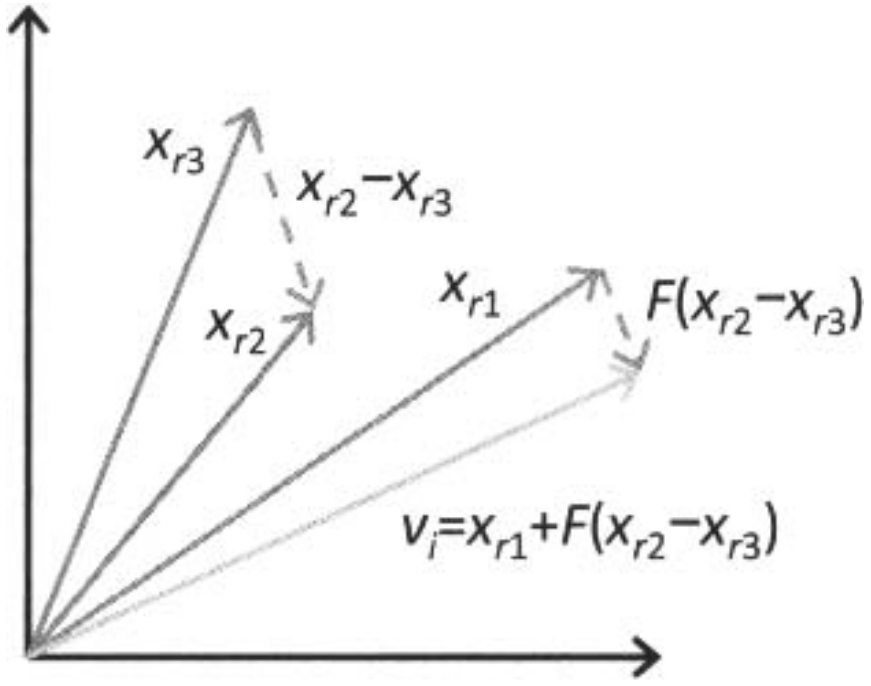
\includegraphics[width=0.5\textwidth]{images/de_beispiel.png}
\end{figure}

\begin{figure}
\caption{Wesentlich DE Algorithmus pseudo-Code. Quelle: \cite{wiley_evolutionary}}
\label{fig:de_pseudo}
\centering
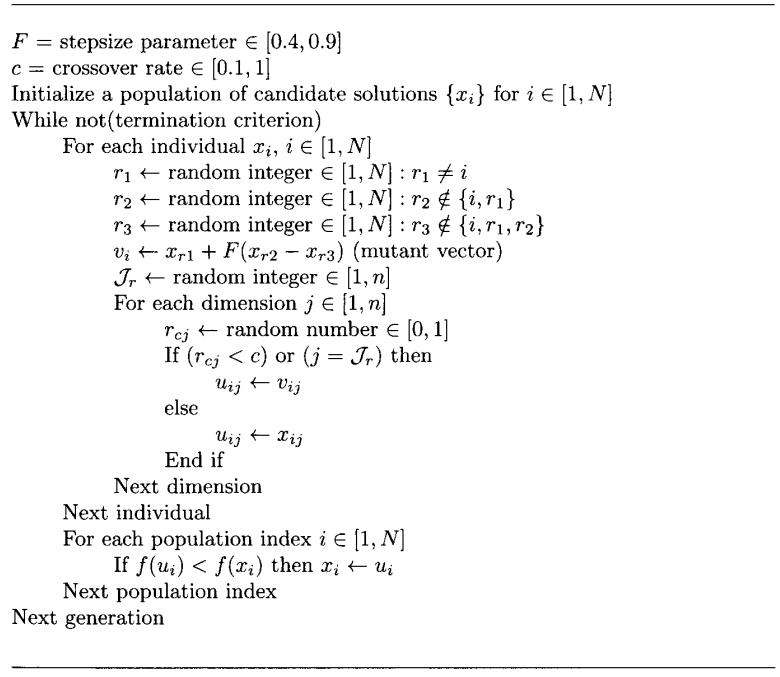
\includegraphics[width=0.5\textwidth]{images/de_pseudo.png}
\end{figure}

Der Algorithmus, den die Abbildung \ref{fig:de_pseudo} beschreibt, wird \enquote{DE/rand/1/bin} genannt und es stellt die einfachste Variante der DE Algorithmen dar. Andere Varianten sind zum Beispiel \enquote{DE/best/1/L}, \enquote{DE/best/2/bin}, \enquote{DE/rand/1/exp}.\par
Jeder Teil dieser Namen bezieht sich auf der Verfahren, die für bestimmte Schritte der DE Algorithmen verwendet werden.\par
Zum Beispiel der \enquote{rand/best}-Teil\footnote{\enquote{best} und \enquote{rand} sind nicht die einzige Varianten.} beschreibt wie Vektoren $x_{r1}$ und $x_{r2}$ im 2. Schritt ausgewählt werden. \enquote{rand} bedeutet, dass die Vektoren zufälligerweise ausgewählt werden, während \enquote{best} heißt, dass die beste Vektoren eine höher Wahrscheinlichkeit haben, um ausgewählt zu werden.\par
In \cite{love_u_mex} werden die Leistungen mehrerer Varianten von DE Algorithmen vergleicht.\par
Wenn Vektoren $x_{r1}$ und $x_{r2}$ zufällig ausgewählt werden, gibt es ein Element der \textbf{Zufälligkeit}. Wenn nur die besten Vektoren ausgewählt werden, wird \textbf{Ausbeutung} gefördert. Die Tatsache, dass nur die beste Vektor im 6. Schritt behaltet wird, zeigt die Verwendung von \textbf{Rückmeldung}. Die Kombination, die im 5. Schritt stattfindet, könnte auch entweder \textbf{Erkundung} oder \textbf{Ausbeutung} fördern.

%------------------------------------------------

\section{Diskussion}
\lettrine[nindent=0em,lines=3]{D} er größte Vorteil der evolutionären Algorithmen ist, dass es praktisch keine Grenze für ihren Verwendungsbereich gibt. Wie vorher gesagt, wenn es eine geeignete Darstellung der Lösungen eines Problems gibt, und eine geeignete Zielfunktion sich definieren lässt, kann jedes Problem mit EA optimiert werden.\par
Ein Nachteil der EA ist, dass die Definition einer geeigneten Zielfunktion ein Problem gleich groß als das ursprüngliche erstellen könnte. Dies ist vermeidbar, indem das Problem geteilt wird. In der Praxis werden oft EA verwendet, um mehrere separate Teile großer komplexer Systemen zu optimieren.\par
Noch ein Nachteil der EA ist, dass die Einstellung des Parametern der Algorithmen auch ein großes Problem darstellen könnte. Die Leistung der Algorithmen ist in großer Maßnahme davon abhängig, wie die ursprüngliche Bevölkerung initialisiert wird, und welche Werte für die Parameter der Algorithmen ausgewählt werden. Dies ist so ein großes Problem geworden, dass dazu Forschung betrieben wird. Um einige Beispiele zu nennen, \cite{pso_tuning_a} und \cite{pso_tuning_c} stellen Verfahren zur Parametereinstellung für PSO vor.\par
EA sollten berücksichtigt werden, immer wenn ein schwieriges Optimierungsproblem gelöst werden soll. Das bedeutet aber nicht, dass EA immer die beste Wahl für den Job sind; Wenn eine Gebäude oder ein komplexes Transportsystem projektieren werden soll, dann sind EA eine geeignete Werkzeug; Wenn eine komplexe elektrische Schaltung oder ein Computerprogramm entwerfen werden soll, dann können die EA die Aufgabe erfüllen; Aber wenn das Problem jedoch mit klassischen Methoden, entweder analytisch oder numerisch, eine gute genug Lösung bietet, ist es besser, diese Methoden zu verwenden.

%------------------------------------------------

\section{Fazit}
\lettrine[nindent=0em,lines=3]{D} ank dem Wachstum des Informatikbereichs und der heutigen Rechnerleistung ist es immer mehr möglich, größer und komplexer Systeme zu entwickeln. Dies bringt auch große und komplexe Herausforderungen mit. EA (und KI insgesamt) sind aber gute Werkzeuge, um diese neue Herausforderungen zu überwinden.\par
Künftig sollen EA in möglichst immer mehr Bereiche eingeführt worden. Ferner sollen wir weiterhin die Natur als Inspiration betrachten. Sowohl in der Wissenschaft, als auch in der Kunst, hat sich die Natur als die beste Muse erwiesen.

%----------------------------------------------------------------------------------------
%	REFERENCE LIST
%----------------------------------------------------------------------------------------

\renewcommand{\refname}{Quellenverzeichnis}
\bibliographystyle{alpha}

\bibliography{quellenverzeichnis}

%----------------------------------------------------------------------------------------

\end{document}
